\colorbox{white!10!}{
    \begin{minipage}{0.2\textwidth}
       \begin{flushleft}
        \includegraphics[width = 0.6\textwidth]{Эмблема.png}
       \end{flushleft}
    \end{minipage}
    \begin{minipage}[t]{0.7 \textwidth}
        \begin{center}
            {\huge \textsc{Красноярская Летняя Школа. Сезон $7^2 - 2$}}
            \vspace{0.25cm}
            
            { \huge \textbf{ФМТ. Тур 4.1}}
        \end{center}
        \vspace{0.05cm}
    \end{minipage}
}

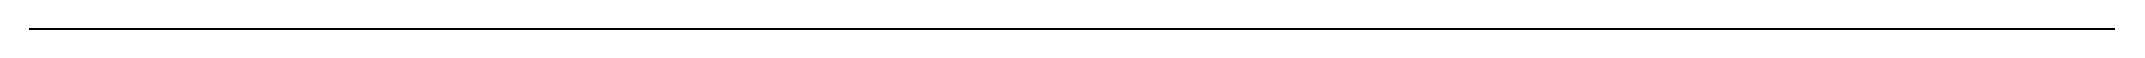
\begin{tikzpicture}
    \draw[thick] (-6.5,0)--(20,0);
\end{tikzpicture}
\begin{enumerate}
    \item По спускающемуся эскалатору бежит вниз пассажир со скоростью $v = 2$ м/с относительно эскалатора. Скорость эскалатора равна $u = 1$ м/с. Количество ступеней эскалатора на спуске $N =90$. Сколько ступеней $N_1$ пройдёт пассажир, спускаясь по эскалатору?
	\item В сосуде с водой плавает кусок льда массой $m$. Система находится в тепловом равновесии. Сколько воды при температуре $t_0 > 0$ нужно добавить в сосуд, чтобы объем выступающей из воды части льда уменьшился в 2 раза? Удельная теплота плавления
    льда $\lambda$, удельная теплоёмкость воды $c_{\text{в}}$.  
\end{enumerate}